\chapter{Part II(c) - Interrupts}

\section{I/O Polling}

I/O Polling is a method used by the CPU to check if any peripheral devices, such as a keyboard or network interface, have data to provide. The CPU continuously monitors each connected I/O device at regular intervals to see if they need attention.
\begin{center}
    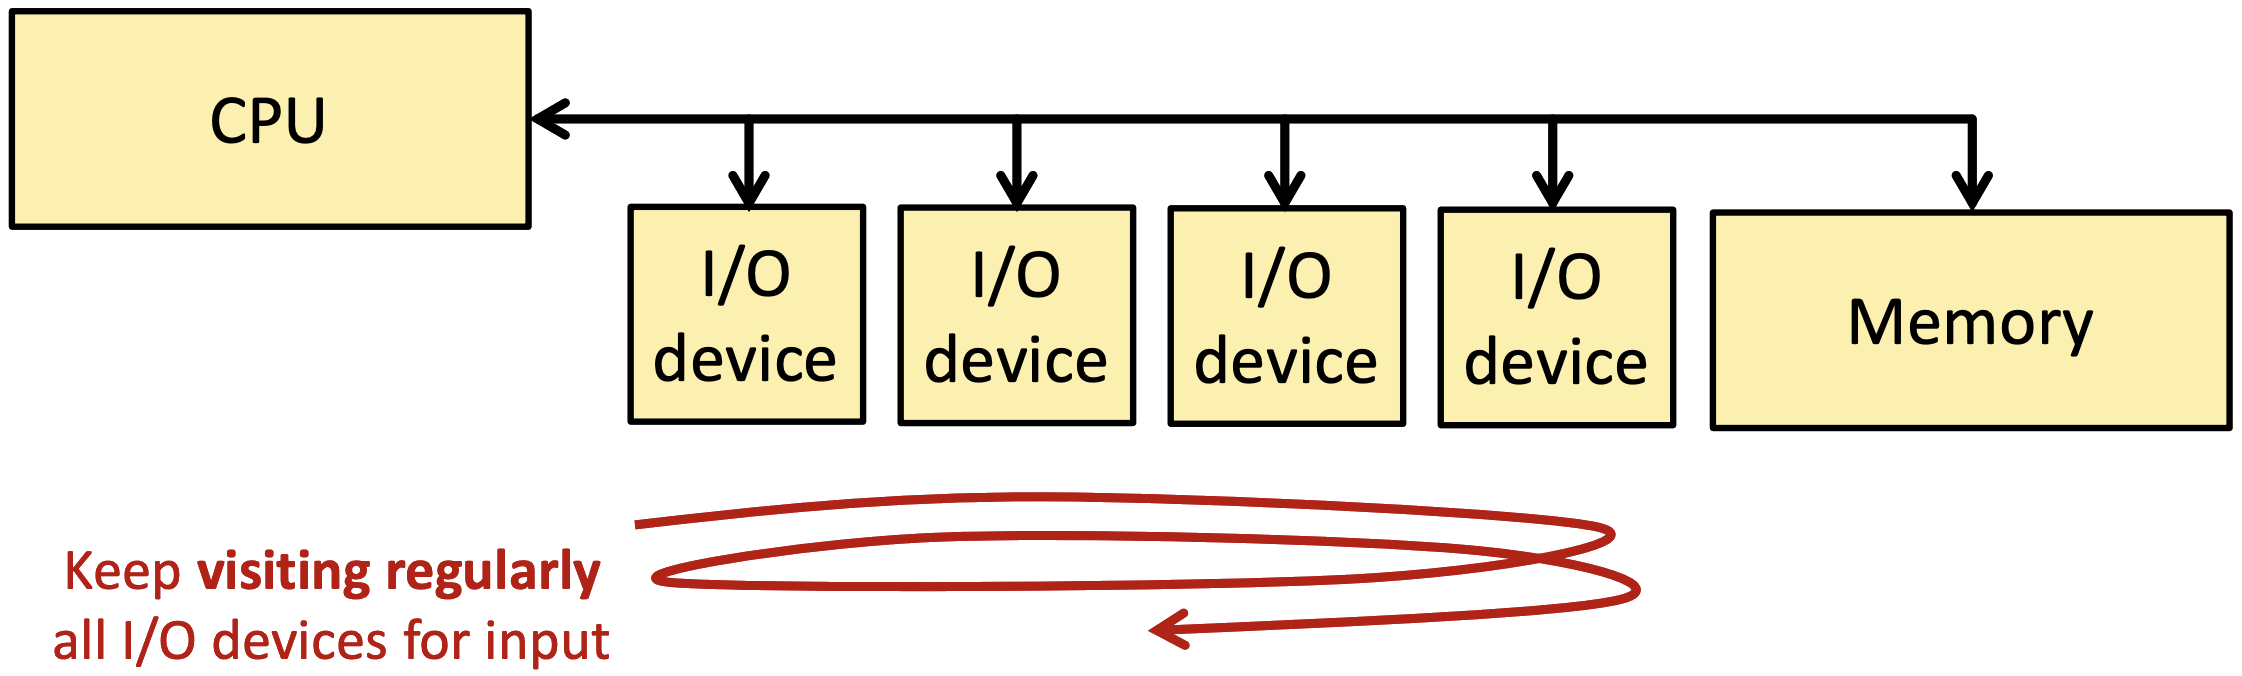
\includegraphics[width=0.65\textwidth]{chapters/chapter2c/images/IOP.png}
\end{center}
\begin{itemize}
    \item[] \textbf{How It Works:} The CPU keeps visiting each I/O device in a loop to check for input or status changes. This is known as "polling" the devices.
    \item[] \textbf{Drawbacks:} This approach can be very resource-intensive. If a device operates at high speed and requires immediate handling, the CPU must check it frequently, which can consume significant processing time.
\end{itemize}

\section{I/O Interrupts}
\textit{Instead of continuously checking the status of peripherals, it is more efficient to have them \textit{request attention} when needed. This approach minimizes CPU usage by eliminating the need for constant polling.}
\begin{itemize}
    \item[-] \textbf{Polling Method:} The CPU checks the status of a peripheral device by repeatedly executing a loop to monitor the peripheral register. This approach requires continuous CPU attention, which can be inefficient in systems with multiple peripherals. \\
    \item[-] \textbf{Interrupt Method:} In an interrupt-driven approach, peripherals alert the CPU only when they need attention. The CPU executes an interrupt service routine (ISR) to handle the request. This method allows the CPU to focus on other tasks until interrupted, improving efficiency.
\end{itemize}

\begin{center}
    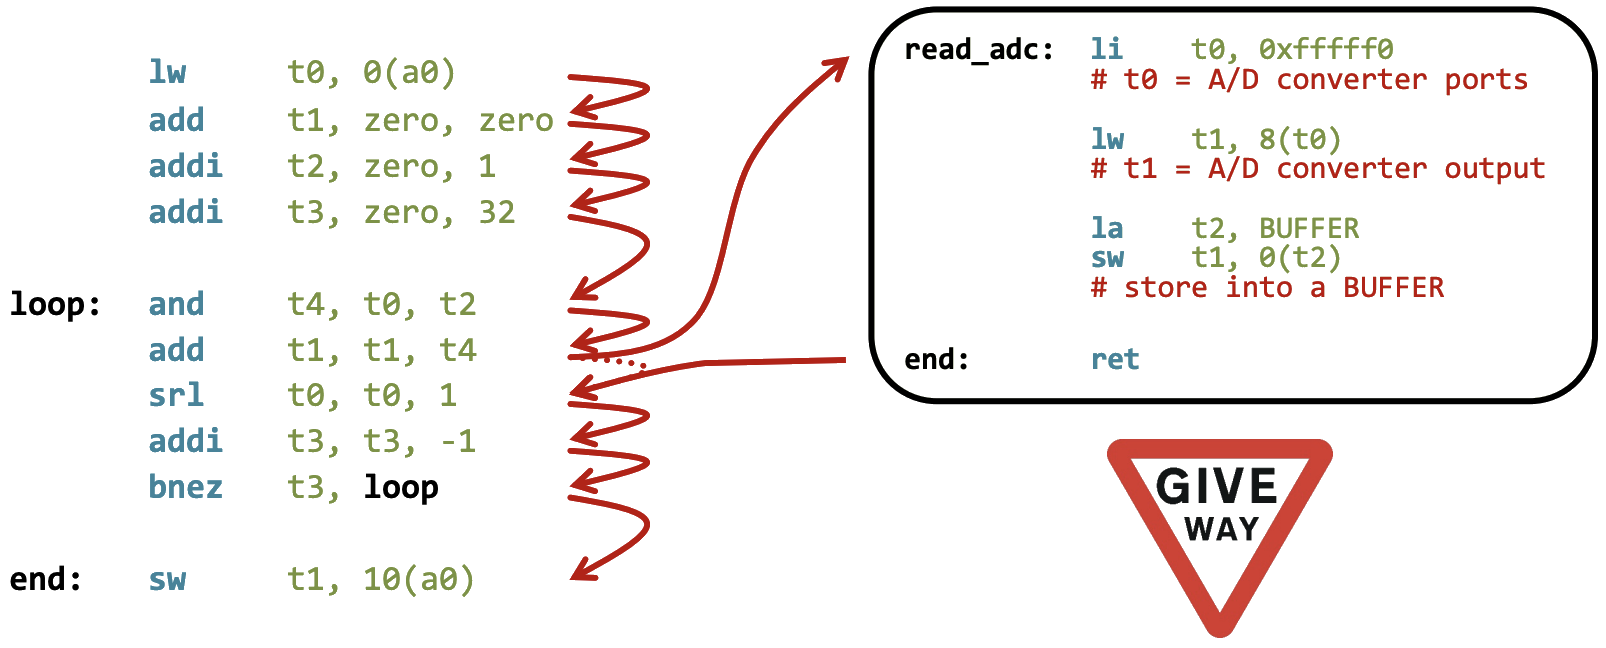
\includegraphics[width=0.65\textwidth]{chapters/chapter2c/images/IOI.png}
\end{center}

\subsection{The Basic Concept of I/O Interrupts}

I/O interrupts provide a mechanism for a controller to handle external requests efficiently by temporarily diverting program execution. \\
\textbf{This is not the actual implementation, but basic concept for you to help you understand what we're aiming for.}
\begin{center}
    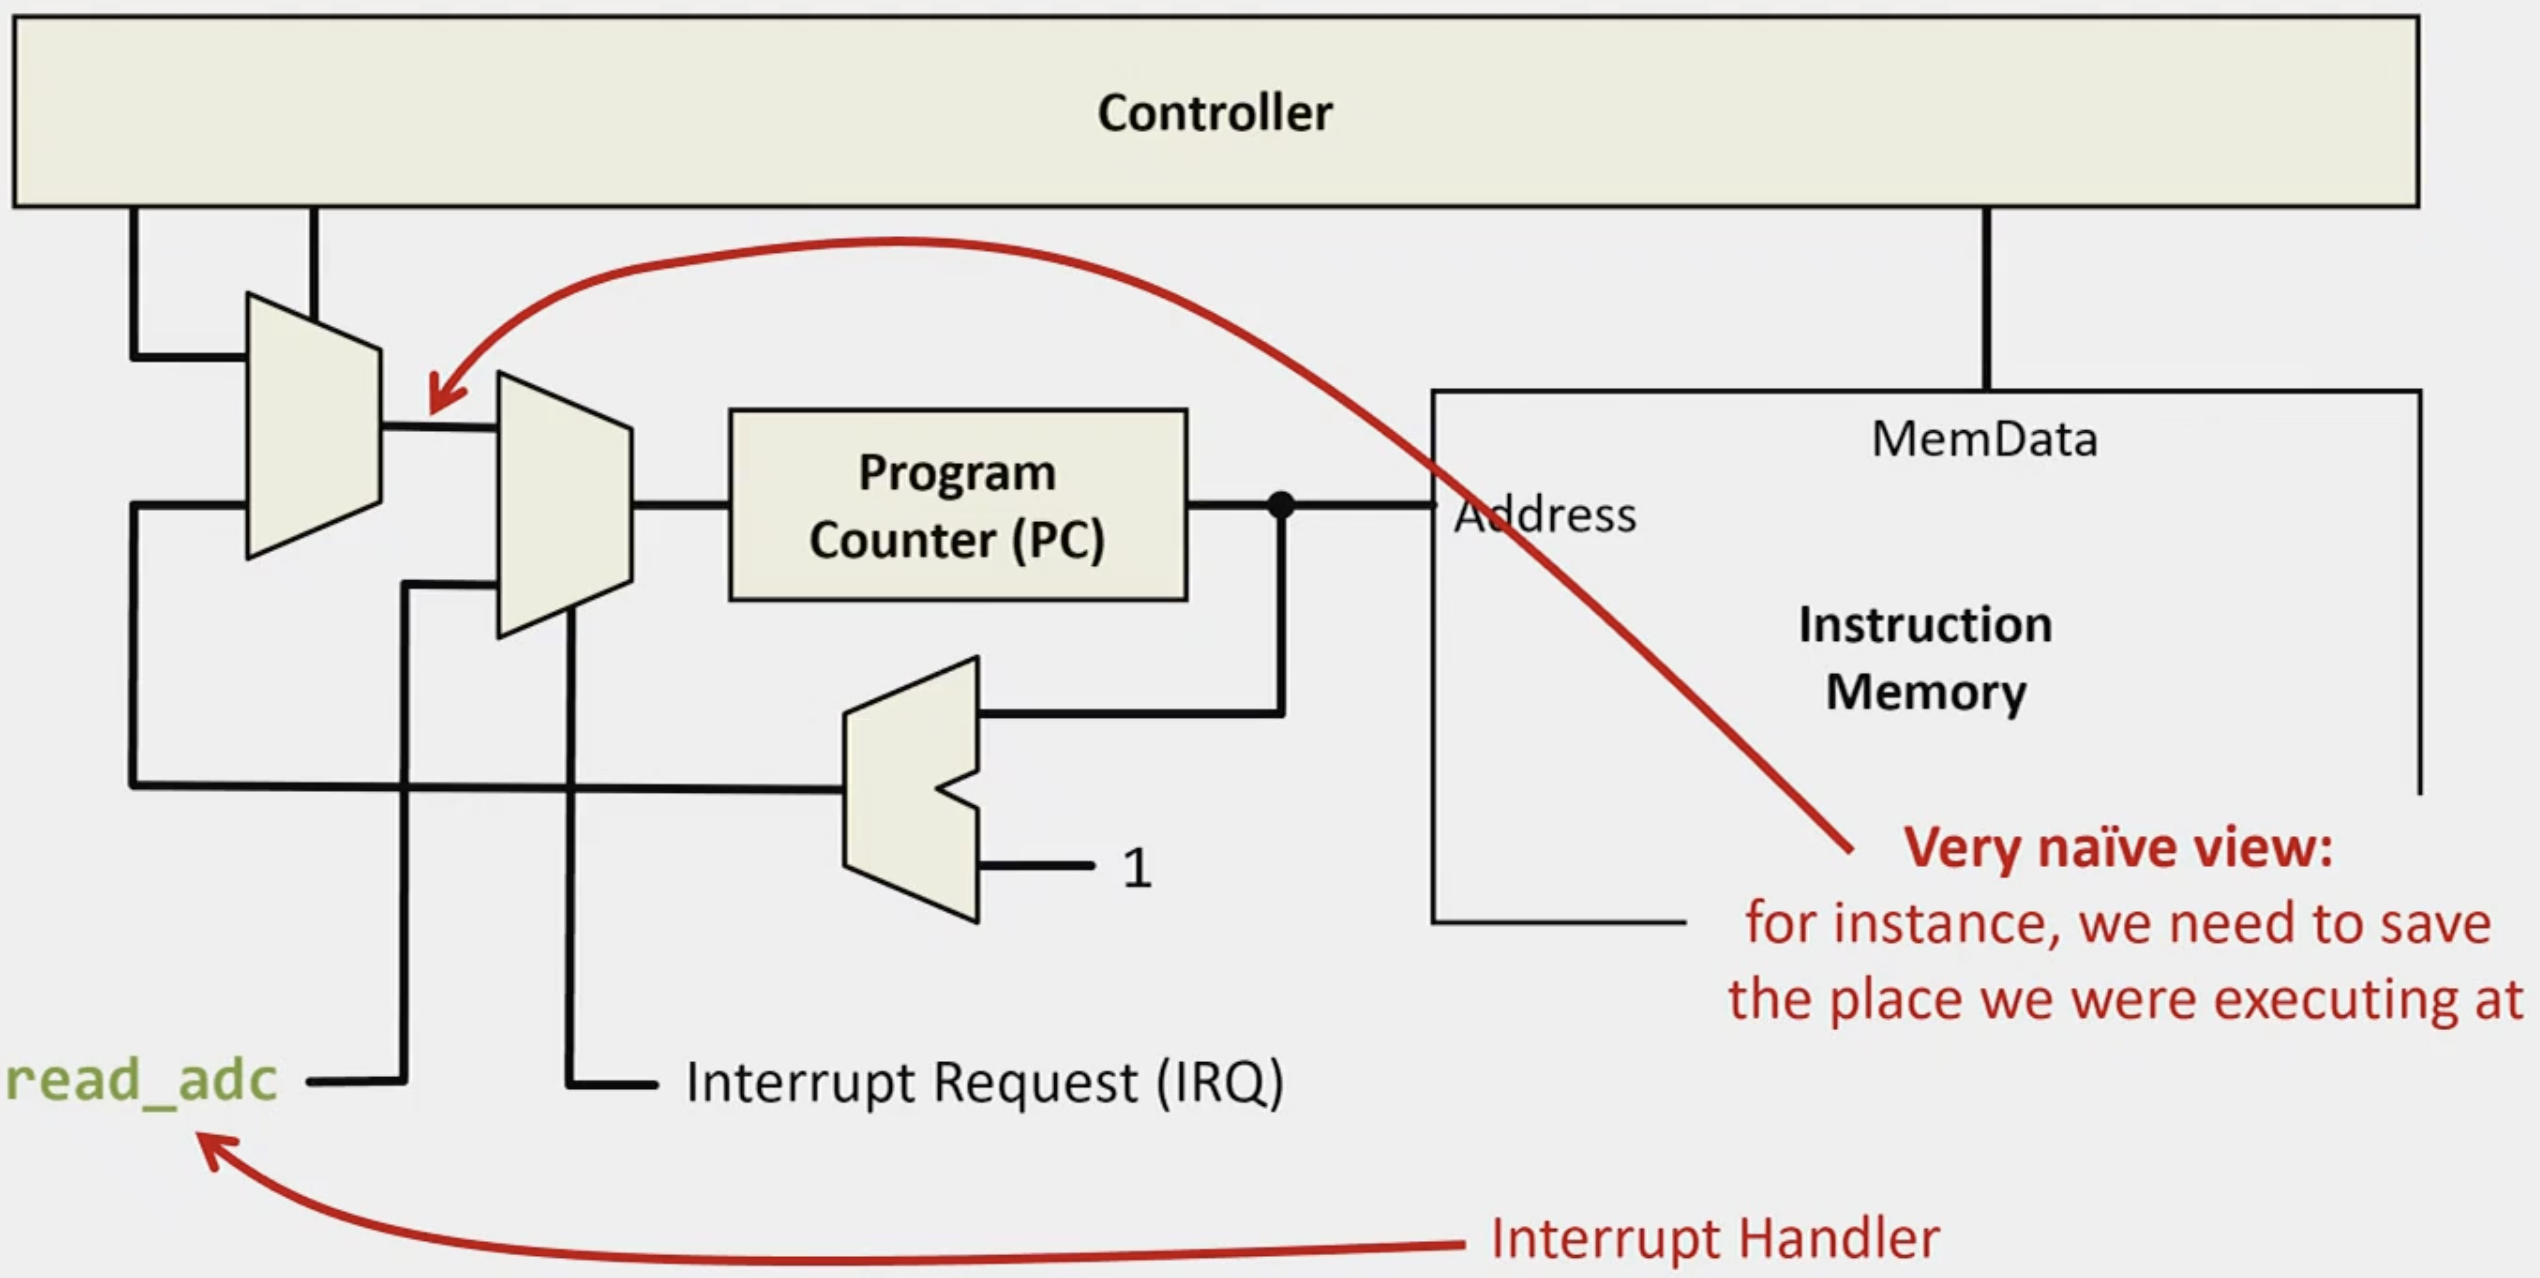
\includegraphics[width=0.65\textwidth]{chapters/chapter2c/images/basic_idea.png}
\end{center}

\begin{itemize}
    \item \textbf{Interrupt Request (IRQ):} An interrupt signal is triggered, typically from an I/O device, to request immediate attention from the controller.

    \item \textbf{Program Counter (PC) Preservation:} The current value of the Program Counter (PC), which holds the address of the next instruction, is saved to allow resumption of normal execution after the interrupt is handled.

    \item \textbf{Interrupt Service Routine (ISR):} The controller redirects the PC to the address of the interrupt handler function, denoted here as \texttt{read\_adc}. This function processes the interrupt by executing specific instructions related to the I/O request.

    \item \textbf{Instruction Memory Access:} The \texttt{Instruction Memory} is accessed to fetch instructions at the new PC address, executing the ISR for the interrupt.

    \item \textbf{Resuming Program Execution:} Once the interrupt has been serviced, the controller restores the saved PC value, allowing the program to continue from the point it was interrupted.
\end{itemize}

\textbf{Considerations for I/O Interrupt Handling} \\
When managing multiple I/O interrupts, several issues must be addressed:

\begin{itemize}
    \item \textbf{Identifying the Source of the Interrupt:} In systems with multiple peripherals, it is essential to determine which device triggered the interrupt. This can be achieved through:
    \begin{itemize}
        \item \textit{Polling:} After an interrupt, the software checks each peripheral sequentially.
        \item \textit{Identification by the Peripheral:} The I/O peripheral itself sends an identification signal.
    \end{itemize}

    \item \textbf{Handling Different Priorities:} Some interrupts may require immediate attention, while others can be delayed. Assigning priorities ensures critical interrupts are serviced promptly, while less urgent ones may wait.

    \item \textbf{Impact on Current Execution:} The system must decide whether to allow the current instruction(s) to complete before handling the interrupt or to pause immediately. This decision impacts program flow and execution timing.
\end{itemize}
\newpage
\subsection{Interrupt Cycle Description}

The interrupt cycle is a sequence where a peripheral device signals an interrupt to the processor, which responds by acknowledging the interrupt and reading the device identifier from the data bus. The following signals are involved in this process:
\begin{center}
    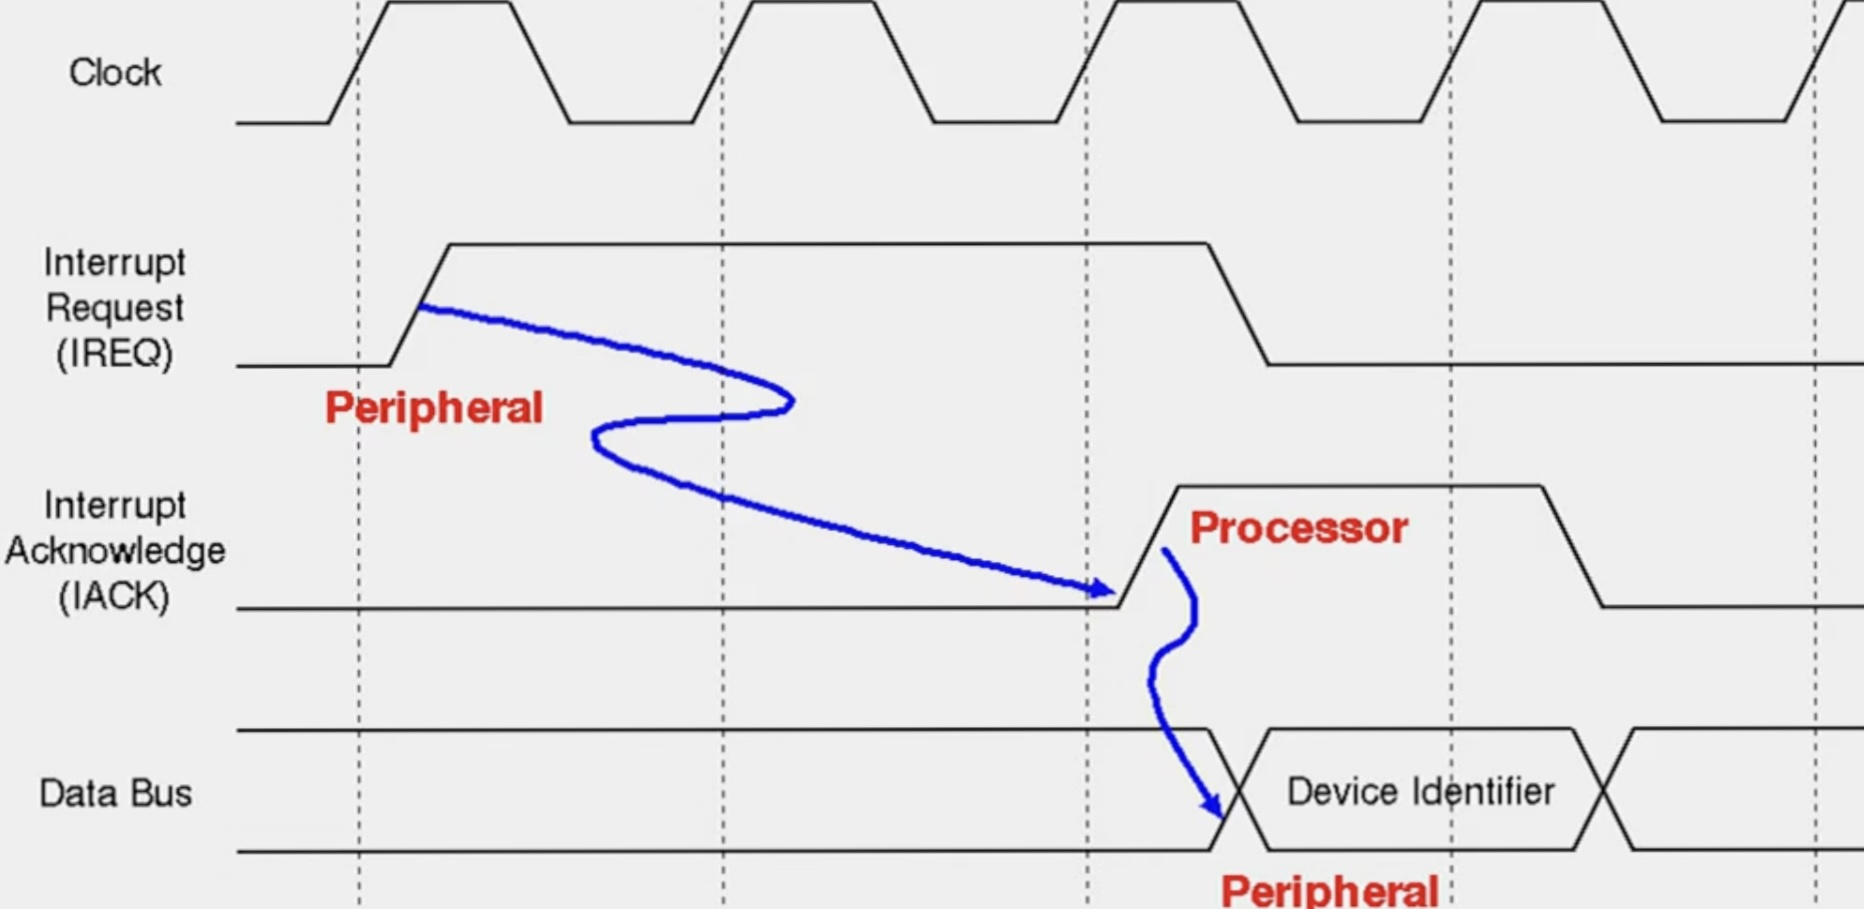
\includegraphics[width=0.65\textwidth]{chapters/chapter2c/images/interrupt.png}
\end{center}
\begin{itemize}
    \item \textbf{Clock Signal}: The clock signal provides the timing for synchronization between the processor and peripherals.
    
    \item \textbf{Interrupt Request (IREQ)}: A peripheral asserts this signal to request service from the processor. When IREQ goes high, the processor detects an interrupt request.
    
    \item \textbf{Interrupt Acknowledge (IACK)}: In response to IREQ, the processor sends an acknowledgment signal (IACK) to the peripheral. This signal indicates that the processor is ready to handle the interrupt.
    
    \item \textbf{Data Bus}: After the IACK signal is asserted, the peripheral places its device identifier on the data bus, allowing the processor to identify the source of the interrupt.
\end{itemize}

The interrupt cycle proceeds as follows:
\begin{enumerate}
    \item The peripheral raises the \textbf{IREQ} line to signal the interrupt request.
    \item The processor detects the interrupt and, after some clock cycles, responds by asserting the \textbf{IACK} line.
    \item The peripheral then places its \textbf{Device Identifier} on the data bus.
    \item The processor reads the device identifier to determine the source of the interrupt and proceeds with the appropriate interrupt service routine.
\end{enumerate}

This cycle ensures that the processor can handle asynchronous requests from peripheral devices in an organized and timely manner.
\newpage
\subsection{I/O Interrupt Priorities: Daisy Chain Arbitration}

Daisy Chain Arbitration is a basic method used to manage I/O interrupt priorities. The process operates as follows:

\begin{itemize}
    \item \textbf{Request Placement:} Any device can initiate a request to access the bus, indicated by signals such as \texttt{IREQ} (Interrupt Request).
    \item \textbf{Acknowledgment Line:} An acknowledgment signal, referred to as \texttt{IACK} or \texttt{Grant}, is sequentially passed from one device to the next.
    \item \textbf{Signal Interception:} The first device that requires access intercepts the acknowledgment signal, preventing it from being passed to devices further down the chain.
\end{itemize}

This method, while simple and easy to implement, has some limitations:
\begin{itemize}
    \item \textbf{Slow Performance:} Due to the sequential nature of signal passing, response times can be slower as the chain length increases.
    \item \textbf{Fixed Priorities:} Devices closer to the bus arbiter have higher priority by design, leading to a rigid priority structure.
\end{itemize}

\begin{center}
    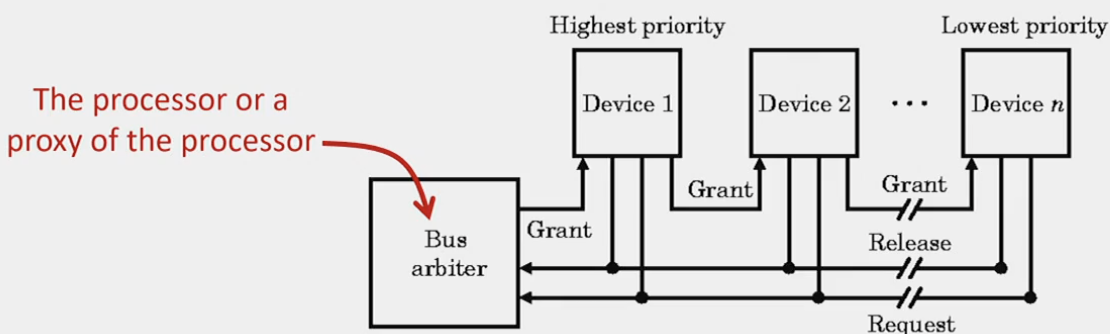
\includegraphics[width=0.75\textwidth]{chapters/chapter2c/images/bus_arbiter.png}
\end{center}

In this setup, the bus arbiter, which acts as the processor or a proxy for the processor, grants access in a priority chain from the highest-priority device to the lowest. This method is suitable for systems where simplicity is valued over flexibility and speed.

\section{Direct Memory Access (DMA)}

Direct Memory Access (\textit{DMA}) is an efficient mechanism designed to offload the processor from managing repetitive and resource-intensive data transfers. Key considerations include:

\begin{itemize}
    \item \textbf{Interrupts Efficiency:} \textit{Interrupts} save the processor from continuously polling Input/Output (I/O) devices, allowing it to focus on computation.
    \item \textbf{Large Data Transfers:} Despite the use of interrupts, the processor may still spend considerable time transferring large chunks of data to and from high-throughput peripherals (e.g., disks, networks).
    \item \textbf{Solution:} A dedicated peripheral, known as the \textit{DMA Controller}, is introduced. This controller autonomously handles data transfers between memory and peripherals (read/write operations), freeing the processor to focus on more critical tasks.
\end{itemize}

\vspace{0.5cm}
\noindent
DMA significantly enhances system performance by reducing processor overhead during data transfer operations.

\vspace{0.8cm}
\begin{center} 
    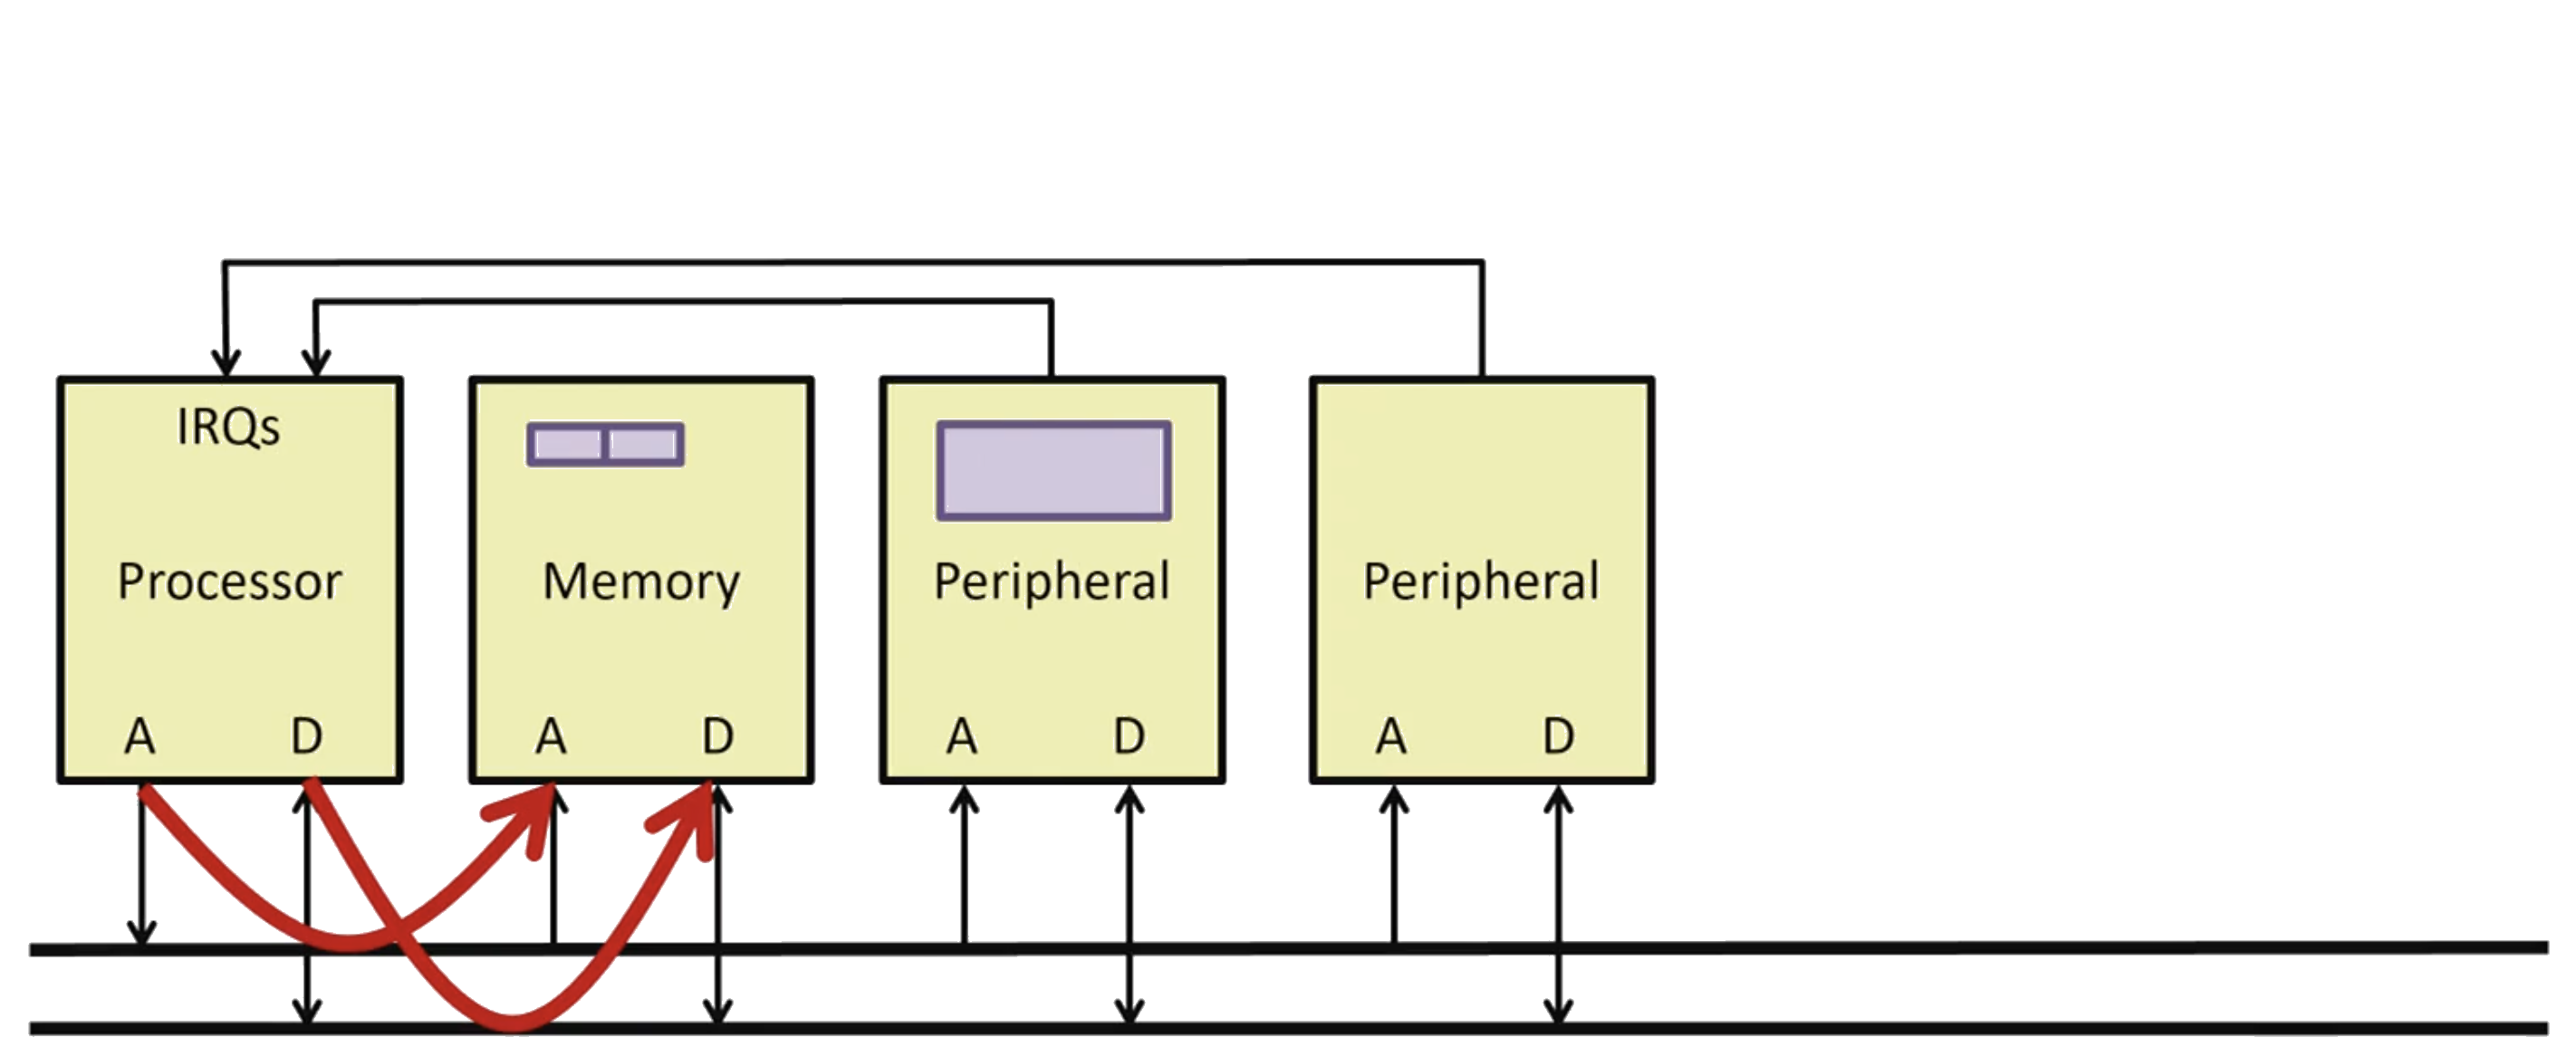
\includegraphics[width=0.65\textwidth]{chapters/chapter2c/images/DMA.png}
\end{center}
\vspace{0.5cm}

The diagram above illustrates a key inefficiency: \textit{using the processor—a complex and expensive machine—to handle simple data transfer operations}. This inefficiency forms the basis for introducing DMA. 

\vspace{1cm}
\begin{center}
    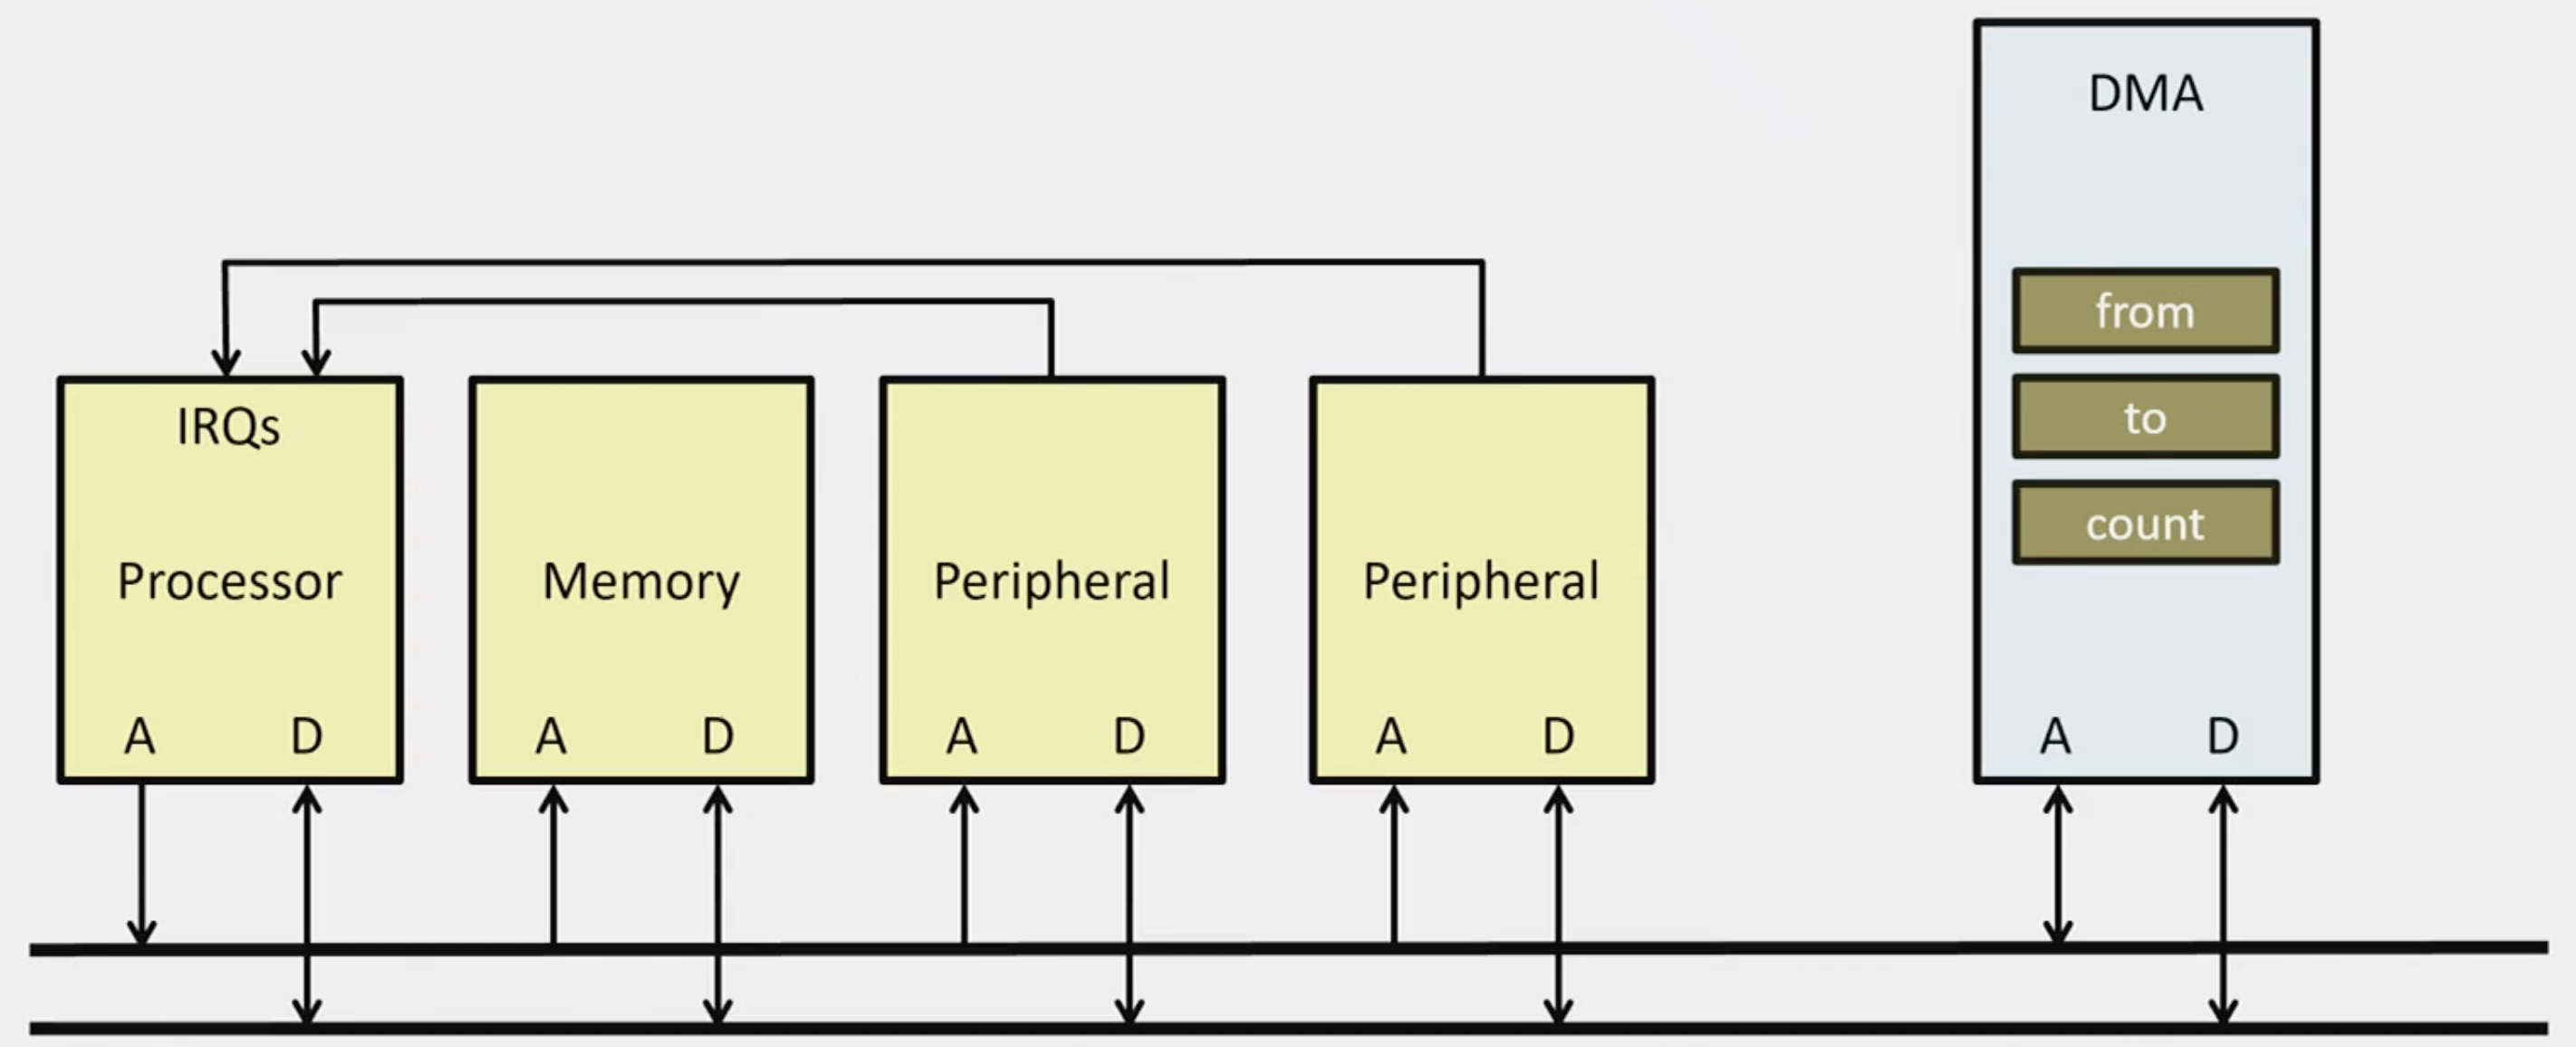
\includegraphics[width=0.65\textwidth]{chapters/chapter2c/images/DMA2.png}
\end{center}
\vspace{0.5cm}

When initiating a data transfer, the \textbf{CPU} communicates with the \textbf{DMA Controller} to start the operation with a specific peripheral. The \textbf{DMA Controller} then handles communication with the \textbf{I/O device}, transferring the data to or from memory. 

\vspace{0.5cm}
\noindent
However, this introduces a new challenge. Previously, the \textit{CPU} was the sole \textbf{master of the BUS}. With the \textbf{DMA Controller} capable of two-way communication with the BUS (on its A input), it also becomes a master of the BUS. This requires a mechanism to manage BUS access between the processor and the DMA Controller.
\vspace{1cm}
\begin{center}
    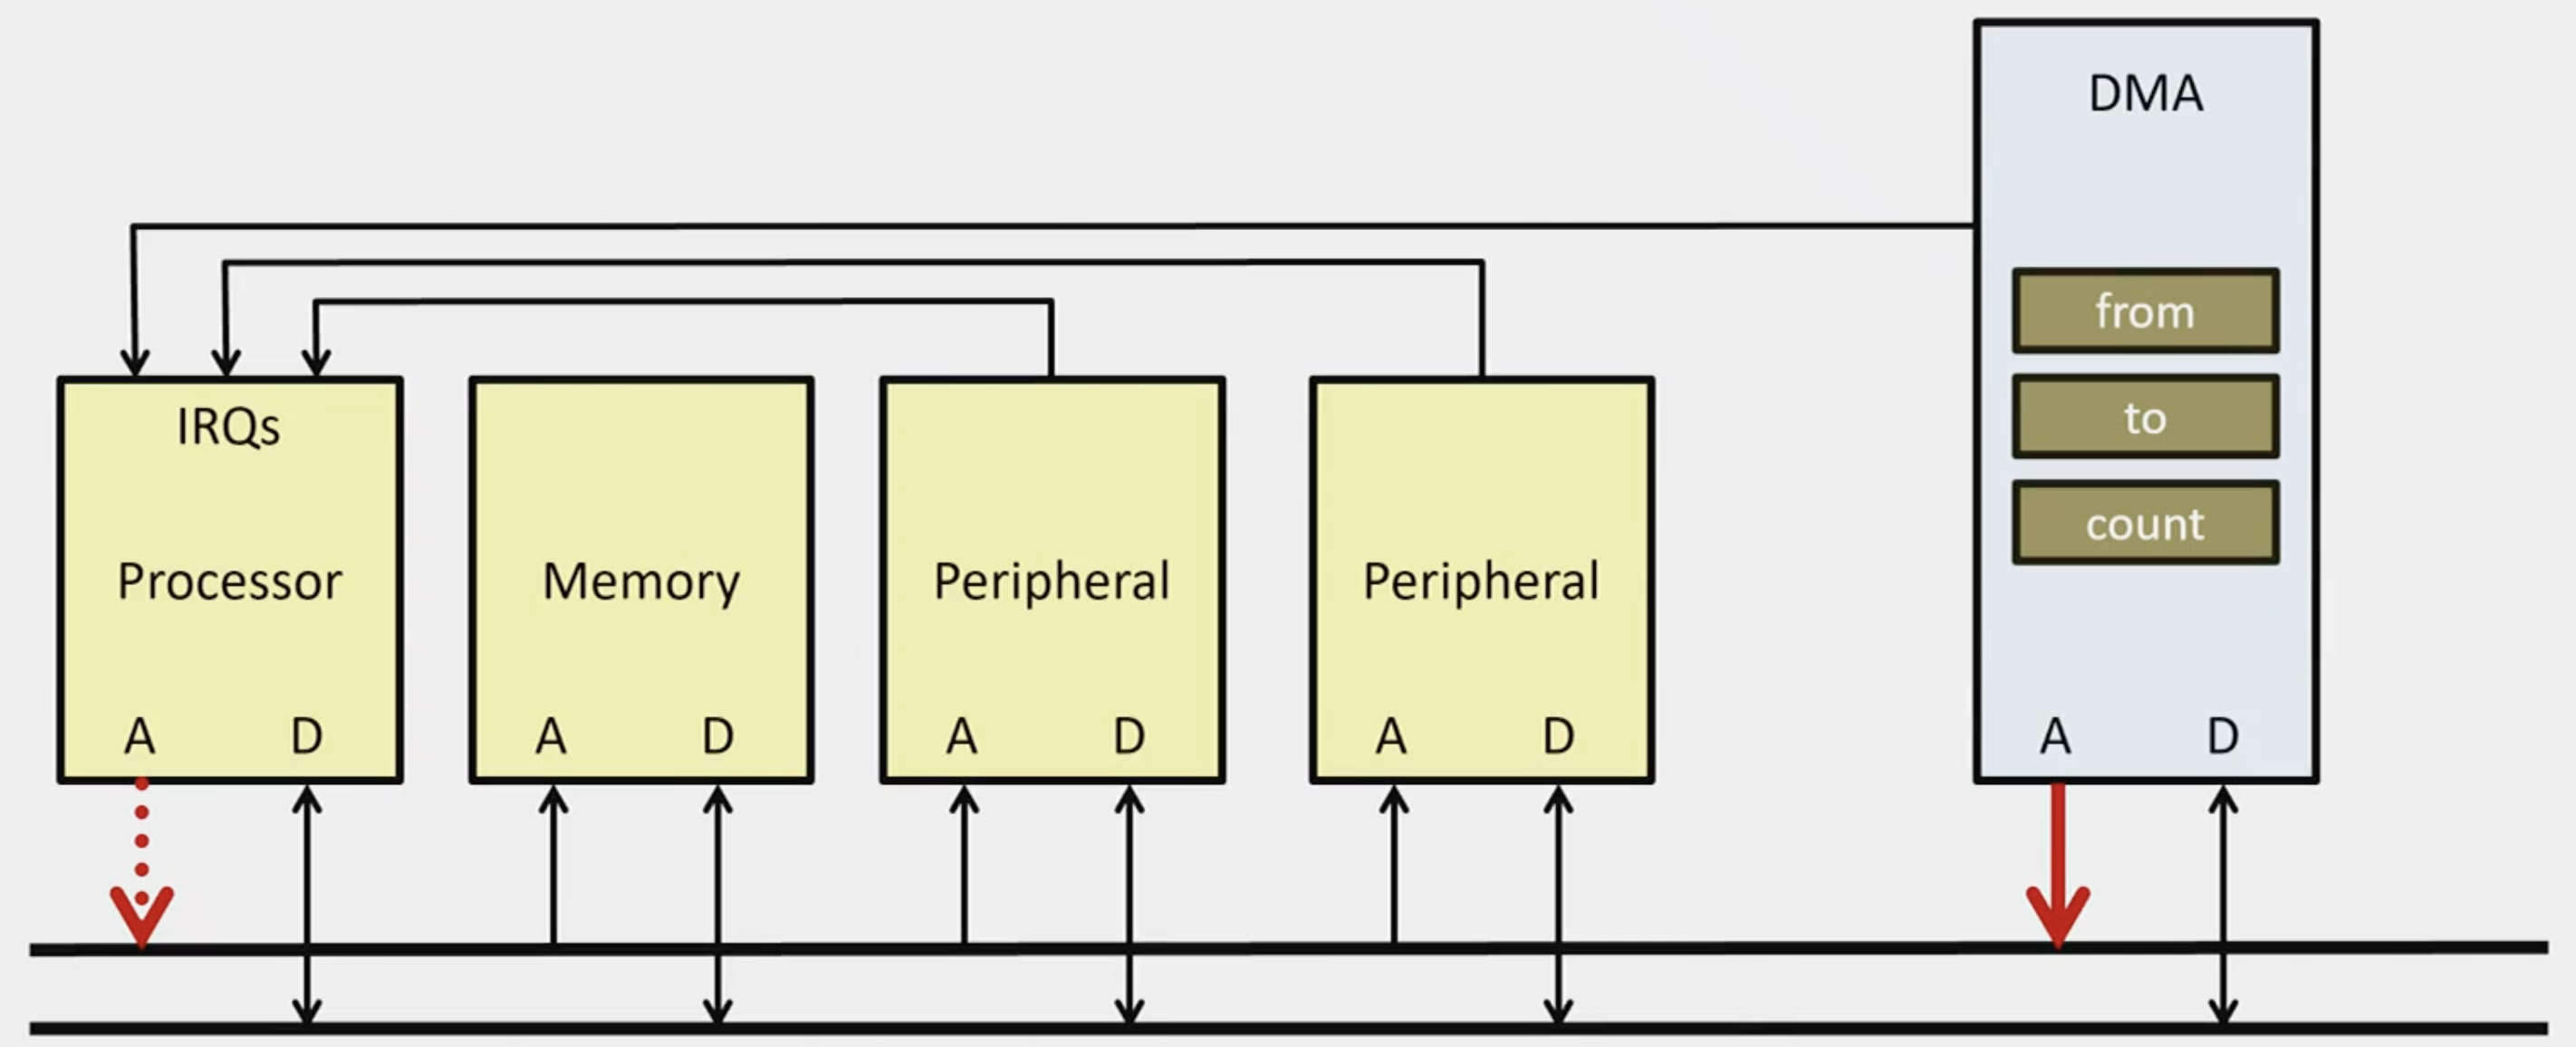
\includegraphics[width=0.65\textwidth]{chapters/chapter2c/images/DMA3.png}
\end{center}
\vspace{0.5cm}
\noindent
This is achieved using a \textbf{Tri-State Buffer}. However, during the data transfer, the processor is temporarily \textit{disconnected from the BUS}, meaning it cannot track the progress of the transfer. Once the transfer is complete, an \textbf{interrupt} is required to notify the processor, ensuring it can resume operations with the updated data.
\newpage
\subsection{Timer and Interrupt Mechanism}

A \textbf{timer} is a critical hardware component used to manage periodic tasks in embedded systems. The timer operates by incrementing a \texttt{count} register until it reaches a programmable \texttt{max} value, at which point it generates an \textbf{interrupt request (IRQ)}. The key features of this mechanism are outlined below:

\begin{center}
    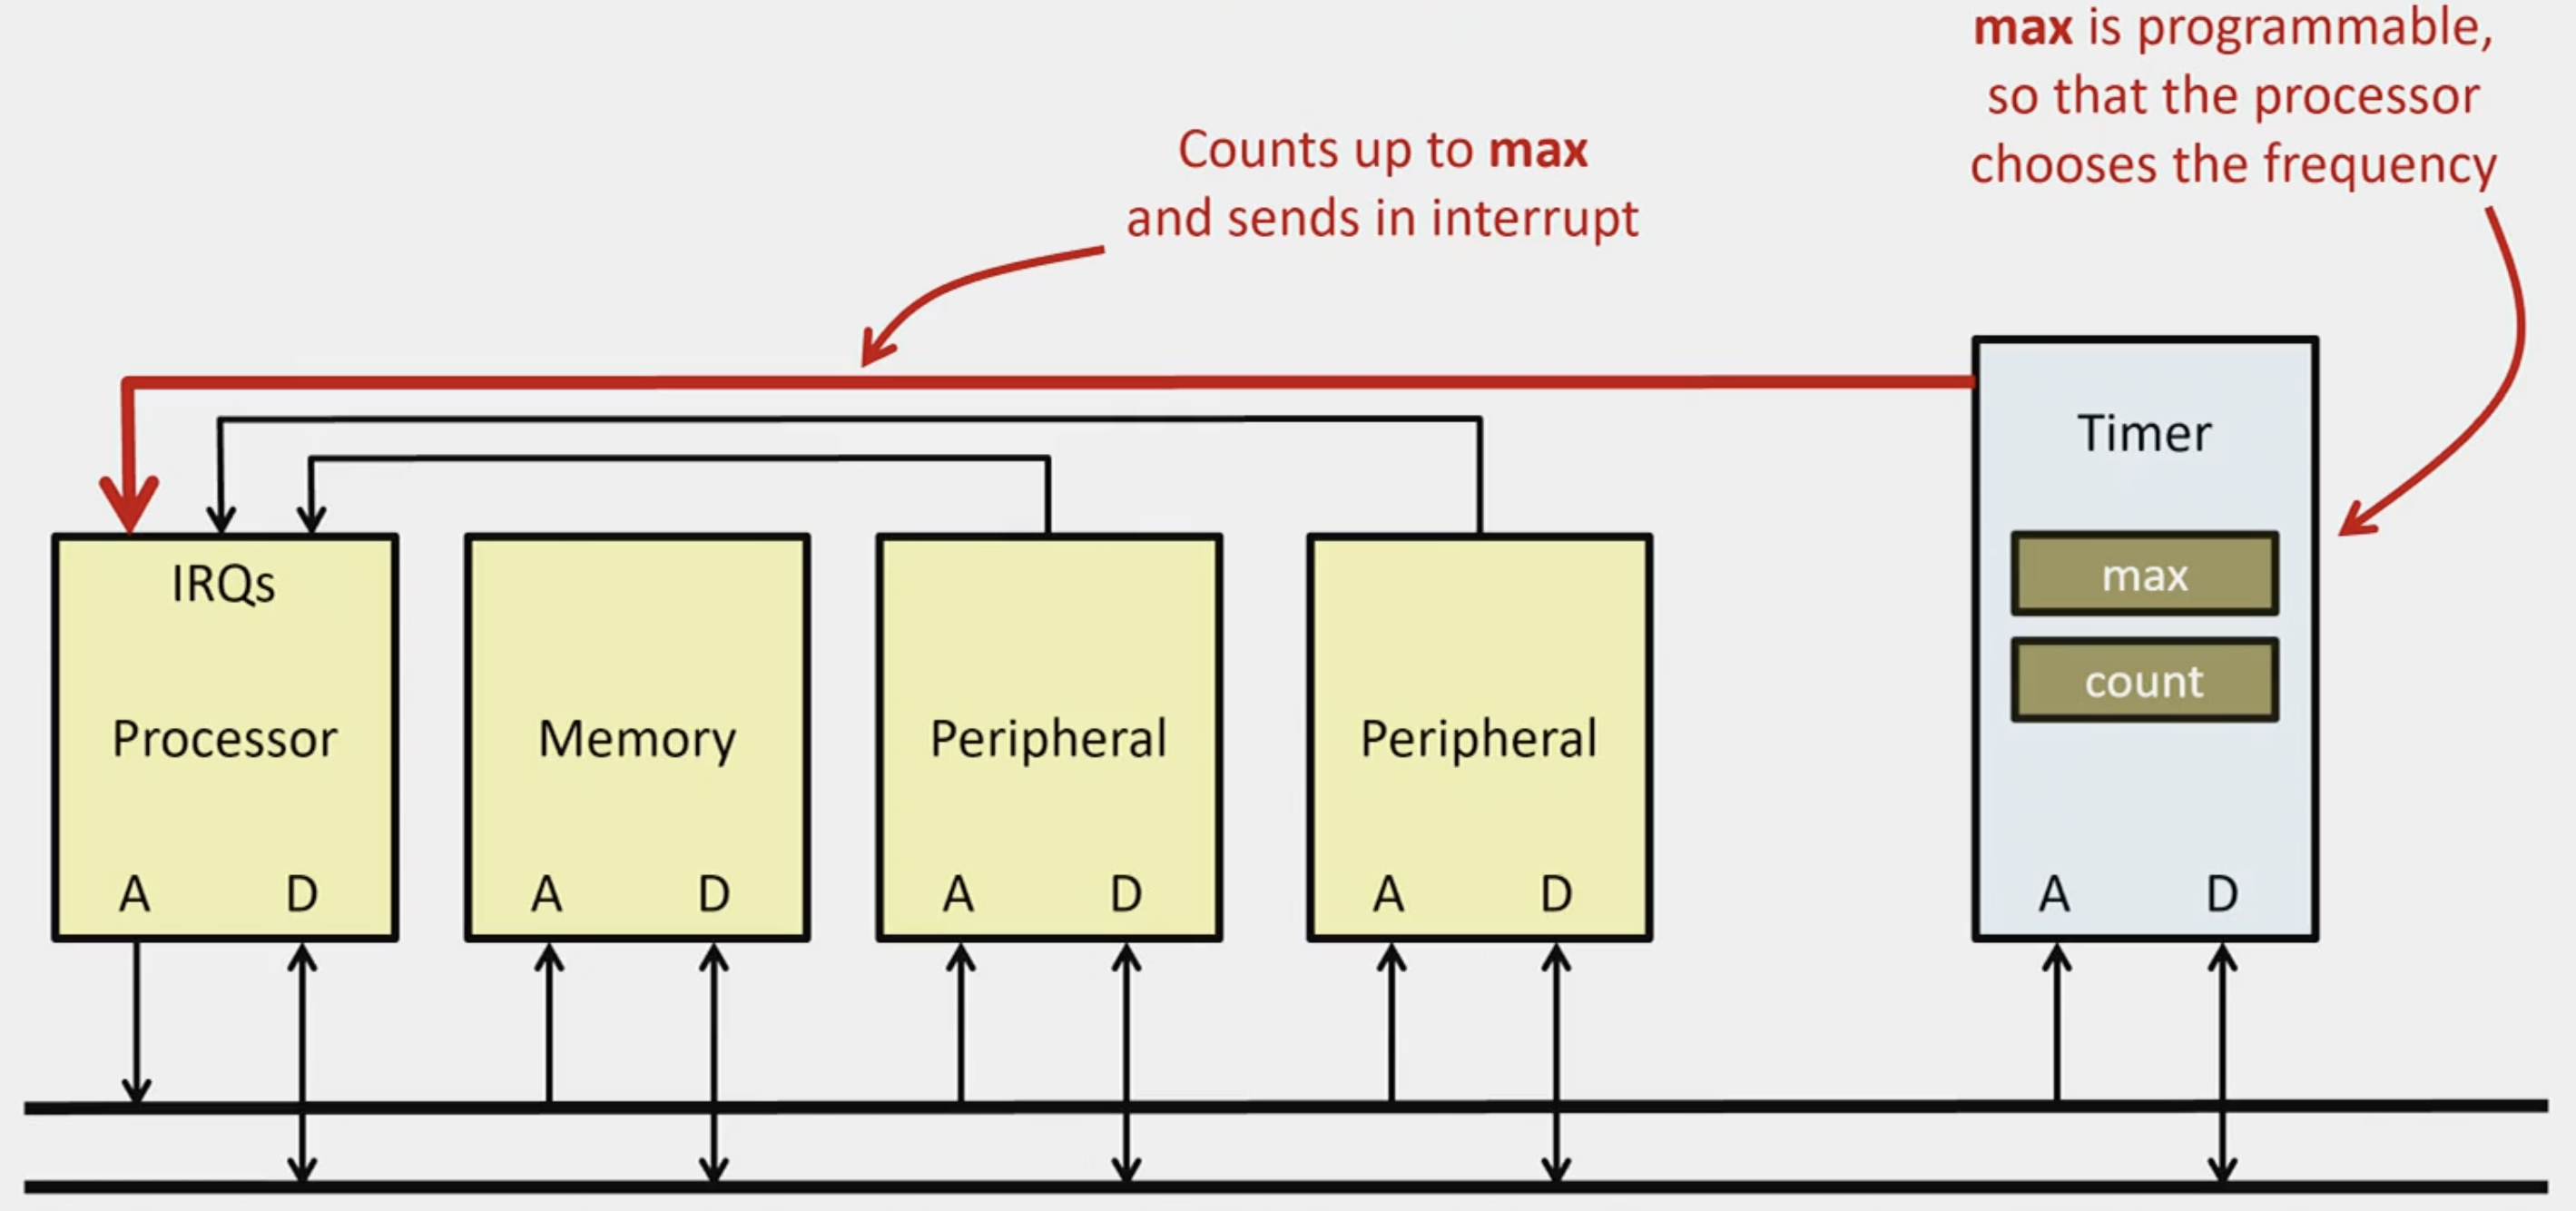
\includegraphics[width=0.65\textwidth]{chapters/chapter2c/images/timer.png}
\end{center}
\begin{itemize}
    \item \textbf{Programmable Frequency:} The \texttt{max} value is configurable, allowing the processor to adjust the interrupt frequency based on system requirements.
    \item \textbf{Interrupt Handling:} Upon reaching the \texttt{max} value, the timer sends an IRQ signal to the processor. This allows the processor to execute specific tasks at regular intervals.
    \item \textbf{System Integration:} The timer interacts with the processor, memory, and peripherals via the system bus, ensuring synchronized operation.
    \item \textbf{Task Management:} Without a timer, it would be impossible for a processor to manage multiple tasks simultaneously, as there would be no mechanism to divide time between different operations. The timer enables multitasking by providing precise time slicing for task scheduling.
\end{itemize}

This mechanism is essential for time-sensitive operations such as task scheduling, event triggering, and real-time control in embedded systems, enabling efficient multitasking and coordination between components.

